\documentclass[11pt]{article}
\usepackage[utf8]{inputenc} % Para caracteres en espa�ol
\usepackage{amsmath,amsthm,amsfonts,amssymb,amscd}
\usepackage{multirow,booktabs}
\usepackage[table]{xcolor}
\usepackage{fullpage}
\usepackage{lastpage}
\usepackage{enumitem}
\usepackage{multicol}
\usepackage{fancyhdr}
\usepackage{mathrsfs}
\usepackage{wrapfig}
\usepackage{setspace}
\usepackage{esvect}
\usepackage{calc}
\usepackage{multicol}
\usepackage{cancel}
\usepackage{graphicx}
\graphicspath{ {pictures/} }
\usepackage[retainorgcmds]{IEEEtrantools}
\usepackage[margin=3cm]{geometry}
\usepackage{amsmath}
\newlength{\tabcont}
\setlength{\parindent}{0.0in}
\setlength{\parskip}{0.05in}
\usepackage{empheq}
\usepackage{framed}
\usepackage[most]{tcolorbox}
\usepackage{xcolor}
\colorlet{shadecolor}{orange!15}
\parindent 0in
\parskip 12pt
\geometry{margin=1in, headsep=0.25in}
\theoremstyle{definition}
\newtheorem{defn}{Definition}
\newtheorem{reg}{Rule}
\newtheorem{exer}{Exercise}
\newtheorem{note}{Note}
\newcommand{\volume}{{\ooalign{\hfil$V$\hfil\cr\kern0.08em--\hfil\cr}}}
\newcommand{\parr}{\mathbin{\|}} % Parralel Symbol
\begin{document}
\setcounter{section}{0}
 \pagestyle{fancy}
\fancyhf{}
\rhead{Section 2: Electromagnetics}
\rfoot{Page \thepage}
\thispagestyle{empty}


\begin{center}
{\LARGE \bf Section 2: Electromagnetics}\\
{\large AE435}\\
Spring 2018
\end{center}
In this section, we will review the basics of charge, electricity, magnetism, and Maxwell equations.
\tableofcontents
\newpage
\section{Electrostatics}
\subsection{Coulomb's Law}
Coulomb's Law is the measure of force between charges. 
\newline
\newline
\newline
\textbf{Case 1: Two Particles}
\newline
\newline
Consider two charges $q_2$ and $q_2$ located at $\vv{r_1}$ and $\vv{r_2}$.
\begin{center}
\vspace{40mm}
\textbf{Figure 1}
\end{center}
The force on $q_1$ due to $q_2$ is
\begin{shaded}
\textbf{Coulomb Force} \newline
\begin{equation}
\vv{F_{12}} = c (\frac{q_1 q_2}{r_{12}^{2}}) \frac{\vv{r_{12}}}{r_{12}} \quad \sim \quad \frac{1}{r^2}
\end{equation}
Where:
\begin{equation*}
\begin{split}
\vv{r_{12}} = \vv{r_1}-\vv{r_2} \qquad &\text{The Sum of Position Vectors} \\
r_{12} = \lvert \vv{r_{12}} \rvert \qquad &\text{The Magnitude of $\vv{r_{12}}$} \\ \\
c = \qquad & \text{Coulomb's Constant} \\
 & = \quad 8.9875x10^9 = \frac{1}{4\pi \epsilon_0} [\frac{N m^2}{c^2}] \\ \\
\epsilon_{0} =  \qquad & \text{Permittivity of Free Space} \\
& = \quad 8.854x10^{-12} [\frac{c^2}{N m^2}]
\end{split}
\end{equation*}
\end{shaded}
Coulomb force scales with the square of the distance as shown by $\sim \frac{1}{r^2}$ in Equation 1.
\newpage
\textbf{Case 2: Many Particles - Coulomb Law}
\newline
\begin{defn} \textbf{Principle of superposition: } \\
Attraction between any pair can be calculated with Equation 1, regardless of the number of particles in the ensemble.
\end{defn}
So, let $\vv{r_i}$ be location of test particle $q_i$. If we have N charged particles, the force on $q_i$ is the linear superposition of the individual forces,
\begin{shaded}
\textbf{Multiple Particle Coulomb Force} \newline
\begin{equation}
\vv{F_{ij}} = \frac{q_i}{4\pi \epsilon_0} \sum_{j \neq i}^{N} q_i \bigg(\frac{\vv{r_{ij}}}{r_{ij}^3}\bigg)
\end{equation}
Where:
\begin{equation*}
\begin{split}
\vv{r_{ij}} = \vv{r_i}-\vv{r_j} \qquad &\text{The vector from test particle $q_i$ to field particle $q_j$} \\
\end{split}
\end{equation*}
\end{shaded}
\newline
\textbf{Case 3: Continuum Generalizations}
\newline \newline
Let us define
\begin{itemize}
\item \textbf{Volume Charge Density} $[\frac{C}{m^3}]$
\begin{equation}
\begin{aligned}
\rho_{e} = \lim_{\Delta \volume \rightarrow 0} \frac{\Delta q}{\Delta \volume}
\end{aligned}
\end{equation}
\item \textbf{Surface Charge Density} $[\frac{C}{m^2}]$
\begin{equation}
\begin{aligned}
\sigma_{e} = \lim_{\Delta \text{S} \rightarrow 0} \frac{\Delta q}{\Delta S}
\end{aligned}
\end{equation}
\end{itemize}
With these, the force acting on charge $q_o$ due to distributed charge sources are:
\begin{shaded}
\textbf{Continuum Charge Coulomb Force} \newline
\begin{equation}
\vv{F_{q_o}} = \frac{q_i}{4\pi \epsilon_0} \Bigg[ \int_{\volume} \frac{\vv{r}-\vv{r}'}{|\vv{r}-\vv{r}'|^3}\rho_{e}(\vv{r}')\mathrm{d}\vv{\volume} + \int_{S}  \frac{\vv{r}-\vv{r}'}{|\vv{r}-\vv{r}'|^3}\sigma_{e}(\vv{r}')\mathrm{d}\vv{S}\Bigg]
\end{equation}
Where:
\begin{equation*}
\begin{split}
\vv{r}' =& \text{ The location within $\volume$ or location on S} \\
\vv{r} =& \text{ The location of $q_o$} \\
\sigma_{e} \text{ and } \rho_{e} =&  \text{ Functions of position $\vv{r}'$} \\
\end{split}
\end{equation*}
\end{shaded}
\newpage
\subsection{Electric Field}
\begin{framed}
\begin{equation}
\vv{E} = \lim_{q_0 \rightarrow 0} \frac{F_{q_o}}{q_o}
\end{equation}
\end{framed}
The force acting on a specific charge $q_o$ from a collection of other charges per unit charge, as the specific charge tends to zero.
\newline
\newline
We set $q_0 \rightarrow 0$ so its presence does not influence the ambient charge.
\newline
\newline
Adding Equation 2 and Equation 5 then dividing thru by q results in:
\begin{shaded}
\textbf{Electric Field Equation} \newline
\begin{equation}
\vv{E} = \frac{q_i}{4\pi \epsilon_0} \Bigg[ \sum_{i=1}^{N} q \frac{\vv{r}-\vv{r_i}}{|\vv{r}-\vv{r_i}|^3} + \int_{\volume} \frac{\vv{r}-\vv{r}'}{|\vv{r}-\vv{r}'|^3}\rho_{e}(\vv{r}')\mathrm{d}\vv{\volume} + \int_{S}  \frac{\vv{r}-\vv{r}'}{|\vv{r}-\vv{r}'|^3}\sigma_{e}(\vv{r}')\mathrm{d}\vv{S}\Bigg]
\end{equation}
Where:
\begin{equation*}
\begin{split}
\vv{E} =& \vv{E}(\vv{r}) \quad \text{ Electric Field is a function of position $\vv{r}$} \\
\end{split}
\end{equation*}
\end{shaded}
We can use integral approach to solve problems, but this can get complex. We can also visualize the Electric Field via field lines, curves that are everywhere tangent to the field.
\newline
\begin{center}
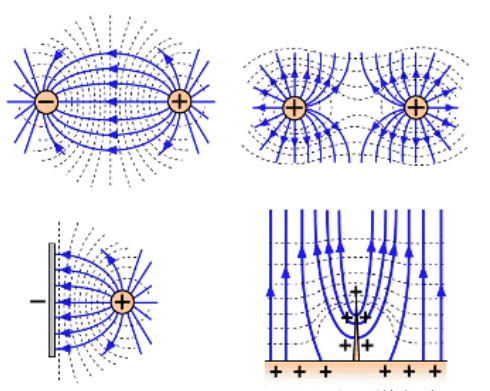
\includegraphics[scale=0.5]{1.png}
\end{center}
\newpage
\subsection{Conductors and Insulators}
\begin{defn} \textbf{Conductor:} Free charges, respond to external Electric field
with charge motion.\end{defn}
\begin{defn} \textbf{Insulator:} Bound charges, no motion. Also often called a
"dielectric"\end{defn}
\subsection{Gauss's Law}
\newline
\begin{defn} \textbf{Gauss's Law:}  Relates the electric field at a surface to the charge enclosed within that surface. The total flux that passes through any closed surface is proportional to the electric charge enclosed by a surface. This surface is the Gaussian Surface.\end{defn}
\textbf{Case 1: Single Charge}
\newline
\newline
The electric field for a single charge is
\begin{framed}
\begin{equation}
\vv{E} = \frac{q}{4\pi \epsilon_0} \frac{\vv{r}}{r^3}
\end{equation}
\end{framed}
If we take the surface integral around an arbitrary volume surrounding the charge we get:
\begin{center}
\vfill
\textbf{Figure 2}
\end{center}
\begin{shaded}
\textbf{Gauss' Law for Electric Fields} \newline
\begin{equation}
\oint_{S} \vv{E}\cdot \hat{n} \, \mathrm{d}A = \frac{q}{4 \pi \epsilon_0} \oint_{S} \frac{\vv{r} \cdot \hat{n}}{r^3} \, \mathrm{d}A
\end{equation}
Where:
\begin{equation*}
\begin{split}
\bigg( \frac{\vv{r}}{r} \bigg) \cdot \hat{n} \, \mathrm{d}A  &= \text{The project of dA on a plane perpendicular to $\vv{r}$} \\
\end{split}
\end{equation*}
\end{shaded}
\newpage
If we divide the projected area, $\bigg( \frac{\vv{r}}{r} \bigg) \cdot \hat{n} \, \mathrm{d}A$, by $r^2$, we arrive at the solid angle $\mathrm{d}\Omega$.
\begin{center}
\vfill
\textbf{Figure 3}
\end{center}
The total solid angle subtended by a surface totally enclosing the charge is $4 \pi$, so 
\begin{equation*}
\oint_{S} \frac{\vv{r} \cdot \hat{n}}{r^3} \, \mathrm{d}A = 4 \pi 
\end{equation*}
As a result, Equation 9 becomes:
\begin{framed}
\begin{equation}
\oint_{S} \vv{E}\cdot \hat{n} \, \mathrm{d}A = \frac{q}{\epsilon_0} 
\end{equation}
\end{framed}
\textbf{Case 2: Many Point Charges}
\newline
\newline
For the case of many point charges, we take the sum:
\begin{equation*}
\oint_{S} \vv{E}\cdot \hat{n} \, \mathrm{d}A = \frac{1}{\epsilon_0} \sum_{i = 1}^{N} qi
\end{equation*}
\textbf{Case 3: Distributed Charge}
\newline
\newline
For a distributed charge, $\rho_e$, we take the integral over the enclosed volume:
\begin{shaded}
\textbf{Integral Form of Gauss's Law} \newline
\begin{equation}
\oint_{S} \vv{E}\cdot \hat{n} \, \mathrm{d}A = \frac{1}{\epsilon_0} \int_{\volume} \rho_e \, \mathrm{d}\volume
\end{equation}
\end{shaded}
\newpage
Also recall Divergence Theorem (also known as Gauss's Theorem):
\begin{shaded}
\textbf{Divergence Theroem} \newline
\begin{equation}
\oint_{S} \vv{F}\cdot \hat{n} \, \mathrm{d}A = \int_{\volume} \nabla \cdot \vv{F} \, \mathrm{d}\volume
\end{equation}
\end{shaded}
which applies to any vector field $\vv{F}$, so we arrive that...
\begin{equation*}
\oint_{S} \vv{E}\cdot \hat{n} \, \mathrm{d}A = \int_{\volume} \nabla \cdot \vv{E} \mathrm{d}\volume = \frac{1}{\epsilon_0} \int_{\volume} \rho_e \, \mathrm{d}\volume
\end{equation*}
\begin{shaded}
\textbf{Differential Form of Gauss's Law} \newline
\begin{equation}
\nabla \cdot \vv{E} = \frac{1}{\epsilon_0} \rho_{e}
\end{equation}
\end{shaded}
\newpage
\subsection{Electrostatic Potential and Energy}
One can show that the curl of the electric field is zero for an electrostatic field. 
\newline
In general $\nabla \times \vv{E} = -\frac{\partial \vv{B}}{\partial t} = 0$ as we will see later.
\begin{equation}
\nabla \times \vv{E} = 0
\end{equation}
We also use the vector identity:
\begin{equation}
\nabla \times \nabla \phi = 0
\end{equation}
\newline
From Equation 14 and Equation 15, we can see the relation $\vv{E}=\nabla \phi$, such that the vector field $\vv{E}$ is related to the gradient in some scalar field.
\newline
\newline
We call $\phi$ the \textbf{electric potential}. And actually use
\newline
\begin{equation}
\vv{E} = - \nabla \phi(\vv{r})
\end{equation}
\newline
For a single point charge $q_i$ at $\vv{r_i}$, by integrating Equation 16, we arrive at:
\newline
\begin{equation*}
\phi(\vv{r}) = \frac{1}{4 \pi \epsilon_0} \frac{q_1}{|\vv{r}-\vv{r_1}|}+\text{constant}
\end{equation*}
\newline
On any curve linking point $P_1$ to point $P_2$ ,
\newline
\begin{equation*}
\phi_{12} (\vv{r}) = \int_{P_i}^{P_2} \nabla \phi (\vv{r}) \cdot \mathrm{d}\vv{l} = - \int_{P_i}^{P_2} \vv{E}(\vv{r}) \cdot \mathrm{d}\vv{l}
\end{equation*}
\newline
Which tells us the work per unit charge to move from $P_1$ to $P_2$.
\newline
More generally,
\newline
\begin{equation*}
\phi(\vv{r}) = \frac{1}{4 \pi \epsilon_0} \Bigg[ \sum_{i=1}^{N} \frac{q_i}{|\vv{r}-\vv{r_i}|} + \int_{\volume} \frac{\rho_e (\vv{r})}{|\vv{r}-\vv{r}'|} \, \mathrm{d}\vv{\volume} + \int_{S}  \frac{\sigma_{e}(\vv{r})}{|\vv{r}-\vv{r}'|} \, \mathrm{d}A'\Bigg]+\text{constant}
\end{equation*}
\newline
Taking line integral from some reference location to $\vv{r}$,
\newline
\begin{equation*}
\int_{\text{ref}}^{\vv{r}} \vv{E}(\vv{r}) \cdot \mathrm{d}\vv{r} = - \int_{\text{ref}}^{\vv{r}} \nabla \phi(\vv{r}) \cdot \mathrm{d}\vv{r} = - \int_{\text{ref}}^{\vv{r}} \mathrm{d}\phi = - \phi (\vv{r})- \phi_{ref}
\end{equation*}
\newline
Now if we set $\phi_{ref} = 0$ at $r \rightarrow \infty$. Then
\newline
\begin{equation}
\phi (\vv{r}) = -\int_{\text{ref}}^{\vv{r}} \vv{E}(\vv{r}) \cdot \mathrm{d}\vv{r}
\end{equation}
\newline
The Potential Energy, $U$, associated with a force $\vv{F}$ is
\newline
\begin{equation*}
U (\vv{r}) = -\int_{\text{ref}}^{\vv{r}} \vv{F}(\vv{r}) \cdot \mathrm{d}\vv{r}
\end{equation*}
\newline
Since $\vv{F} = q \vv{E}$ for electrostatic force as seen in Equation 16, the electrostatic potential is
\newline
\begin{shaded}
\textbf{Electrostatic Potential} \newline
\begin{equation}
\phi (\vv{r}) = \frac{U (\vv{r}) }{q}
\end{equation}
\newline
The electrostatic potential defines the potential energy per unit charge.
\end{shaded}
\newline
If we define $\phi (\infty) = 0$ then $U (\vv{r}) $ is the energy required to bring a test charge from $\vv{r} = \infty$ to $\vv{r}$.
\newpage
\subsection{Poisson and Laplace Equations}
For a charge distribution $q (\vv{r})$:
\newline
\begin{equation}
\phi(\vv{r}) = \frac{1}{4 \pi \epsilon_0} \int \frac{\partial q}{|\vv{r}-\vv{r}'|}
\end{equation}
\newline
Such that
\newline
\begin{equation}
\vv{E}(\vv{r}) =  \frac{1}{4 \pi \epsilon_0} \int \frac{(\vv{r}-\vv{r}') \, \mathrm{d} q}{|\vv{r}-\vv{r}'|^3}
\end{equation}
\newline
\newline
Since $\vv{E} = -\nabla \phi$ from Equation 16. We can solve for $\phi(\vv{r})$ and $\vv{E}(\vv{r})$ if we know $q(\vv{r})$ charge distribution. Alternatively, we can start with the differential form of Gauss's law (Equation 13) and Equation 16,
\newline
\begin{equation*}
\begin{align}
\nabla \cdot \vv{E} = \frac{\rho_e}{\epsilon_o} \qquad &\text{and} \qquad \vv{E} = - \nabla \phi \\ \\
\nabla \cdot (- \nabla & \phi) = \frac{\rho_e}{\epsilon_o} \\ \\
\text{Use laplacian: }& \nabla^2 = \nabla \cdot \nabla \rightarrow 
\end{align}
\end{equation*}
\begin{shaded}
\textbf{Poisson Equation} \newline
\begin{equation}
\nabla^2 \phi = -\frac{\rho_e}{\epsilon_o}
\end{equation}
Where:
\begin{equation*}
\begin{split}
\rho_e &= \rho_e (\vv{r}) \qquad \text{charge density distribution} \\
\phi &= \phi (\vv{r})  \qquad \text{electric potential distribution} \\
\end{split}
\end{equation*}
The Poisson Equation relates charge density distribution $\rho_e (\vv{r})$ to electric potential $\phi (\vv{r})$ distribution.
\end{shaded}
\newline
Alternatively,
\begin{shaded}
\textbf{Laplace Equation} \newline
\begin{equation}
\nabla^2 \phi = 0
\end{equation}
For region with no free (space) charge $\rho_e = 0$
\end{shaded}
\newpage
\section{Electrostatics with Dielectric Media}
\subsection{Polarization}
Many molecules have a positive end and a negative end.
\newline
\newline
Water, H$_{2}$O, for example is a "polar molecule".
\begin{center}
\vspace{30mm}
\textbf{Figure 4}
\end{center}
Oxygen gets slightly more than its share of the electron cloud while hydrogen gets less.
\newline
\newline
Water is an example of a "polar molecule". It is always polarized, even without any electric field present. But even non-polar atoms/molecules can become polarized in an electric field. Polarized, meaning a redistribution of the electron cloud creating an asymmetric charge distribution that aligns with the electric field.
\newline
\newline
We model this by thinking of each polarized atom/molecule as a dipole.
\begin{center}
\vfill
\textbf{Figure 5}
\end{center}
\newpage
Polarization (how skewed the electron cloud is) depends on $\vv{E}$. However, part of $\vv{E}$ is produced by polarization. In addition, the redistribution of charge in a dielectric (insulator) can affect the external charge distribution, which changes $\vv{E}$. In short, we have a non-linear system!
\newline
\newline
A dipole is two equal and opposite charges, $\pm q$, separated by small distance, $\vv{l}$.
\begin{center}
\vfill
\textbf{Figure 6}
\end{center}
We start by defining the dipole potential field.
\begin{shaded}
\textbf{Dipole Potential Field} \newline
\begin{equation}
\phi(\vv{r}) =  \frac{q}{4 \pi \epsilon_0} \frac{(\vv{r}-\vv{r}')}{|\vv{r}-\vv{r}'|^3} \cdot \vv{l}
\end{equation}
\newline
Note: We ignore the higher order terms in $\vv{l}$.
\end{shaded}
This equation is exact for a point dipole, where $|\vv{l}| \rightarrow 0$ as $q \rightarrow 0$. All nonlinear terms vanish for a point dipole, which has no net charge or spatial extent, and has a constant dipole moment.
\newline
\begin{equation}
\vv{p} = \lim_{l \rightarrow 0} q \vv{l} = \text{constant}
\end{equation}
\newline
For dielectric media, we can generalize this to
\newline
\begin{equation*}
\Delta \vv{p} = \int_{\volume} \vv{r} \, \mathrm{d}q
\end{equation*}
\newline
which is the dipole moment of charge distribution in a small volume.
\newpage
Usually, it is more convenient to work with the dipole moment per unit volume
\begin{shaded}
\textbf{Polarization of the Dielectric} \newline
\begin{equation}
\vv{P} = \lim_{\Delta \volume \rightarrow 0} \frac{\Delta \vv{p}}{\Delta \volume}
\end{equation}
\newline
This is a point property, $\vv{P} (\vv{r})$ unit [C/m3], called the Polarization of the dielectric. It's a vector with direction defined by charge separation.
\end{shaded}
\begin{center}
\vfill
\textbf{Figure 7}
\end{center}
Another way to think of this is through physical molecules, rather than just point dipoles:
\newline
\begin{equation}
\begin{align}
\vv{p_m} = \text{Polarization of a Molecule} \\
\vv{P} = N \vv{p_m} \quad \big[\frac{\#}{m^3}\big]
\end{align}
\end{equation}
\newline
where $N$ is the number density of molecules in a dielectric.
\newpage
\subsection{Surface and Volume Charge Density}
Charge displacement due to induced dipoles results in a net surface charge density
\begin{shaded}
\textbf{Net Surface Charge Density} \newline
\begin{equation}
\sigma_p = \vv{P} \cdot \hat{n} \qquad \bigg[\frac{c}{m^2}\bigg]
\end{equation}
\end{shaded}
and a net volume charge density.
\begin{shaded}
\textbf{Net Volume Charge Density} \newline
\begin{equation}
\rho_p = -\nabla \cdot \vv{P} \qquad \bigg[\frac{c}{m^3}\bigg]
\end{equation}
\end{shaded}
\begin{center}
\textbf{The rest of this section will be spend proving Equation 27 and Equation 28.}
\end{center}
\newline
\newline
Consider the boundary of a dielectric shown below. Assume all positive charges in the slab move a displacement vector $\vv{S}$ in response to an applied electric field, $\vv{E}$, and that negative charges are stationary.
\begin{center}
\vfill
\textbf{Figure 8}
\end{center}
\newpage
We find that the differential volume defined by displacement $\vv{S}$ and projected area $\mathrm{d}\vv{A} = \hat{n} \, \mathrm{d}\vv{A}$ is:
\begin{equation*}
\mathrm{d}\volume = \vv{s} \cdot \mathrm{d}\vv{A}
\end{equation*}
If N is the number of positive charges per unit volume in the medium, the charge crossing $\mathrm{d}\vv{A}$ is:
\begin{equation*}
\mathrm{d}q = N q \vv{s} \cdot \mathrm{d}\vv{A}
\end{equation*}
\newline
Recall polarization per molecule (Equation 24) $\qquad \, \, \, \, \vv{p_m} = q \, \vv{s}$
\newline
\newline
And polarization per unit volume (Equation 26) $\qquad \vv{P} = N \, \vv{p_m}$
\newline
\newline
\newline
So charge crossing $\mathrm{d}\vv{A}$,
\newline
\begin{equation*}
\mathrm{d}q = \vv{P} \cdot \mathrm{d}\vv{A}
\end{equation*}
\begin{framed}
Then the \textbf{Net Surface Charge} is the charge per unit area:
\newline
\begin{equation}
\frac{\mathrm{d}q}{\mathrm{d}A} = \sigma_p = \vv{P} \cdot \hat{n}
\end{equation}
\newline
So whenever $\vv{P}$ and $\hat{n}$ are in the same direction, we get a net positive (+) surface charge. Whenever $\vv{P}$ and $\hat{n}$ are in the opposite direction, we get a net negative (-) surface charge.
\end{framed}
\newline
\newline
Similar for Volume Charge Density
\newline
Again, the charge flow out of any surface $\mathrm{d}A$ with normal $\hat{n}$ is:
\newline
\begin{equation*}
\mathrm{d}q = \vv{P} \cdot \mathrm{d}\vv{A} = \vv{P} \cdot \hat{n} \, \mathrm{d}A
\end{equation*}
\newline
So the net flow out of a differential volume equals the total flux integrated over the surface,
\newline
\begin{equation*}
\int_{S} \vv{P} \cdot \mathrm{d}\vv{A} = \int_{S} \frac{\mathrm{d}q}{\mathrm{d}A} \, \mathrm{d}A
\end{equation*}
\newline
No charge is created or destroyed, so the differential loss of charge within $\mathrm{d} \volume $ is:
\newline
\begin{equation*}
- \int_{S} \mathrm{d}q = \int_{\volume} \rho_p \, \mathrm{d}\volume = - \int_{S} \vv{P} \cdot \mathrm{d}\vv{A} = - \int_{\volume} \nabla \cdot \vv{P} \, \mathrm{d}\volume
\end{equation*}
\newline
Thus, similar to Gauss' Law, you get a differential form valid for any arbitrary volume.
\begin{framed}
Then the \textbf{Net Volume Charge} is the charge per unit volume:
\newline
\begin{equation}
\rho_p = -\nabla \cdot \vv{P}
\end{equation}
\newline
So, a negative gradient in polarization creates a positive volumetric charge. Meanwhile, a positive gradient in polarization creates a negative volumetric charge.
\end{framed}
\newpage
\subsection{Gauss' Law for Dielectrics}
Starting with the free-space Gauss's law, we add dielectric charges
\newline
\begin{shaded}
\textbf{Gauss' Law with Dielectric Charges} \newline
\begin{equation}
\begin{aligned}
\oint_{S} \vv{E} \cdot \mathrm{d}\vv{A} = \int_{\volume} \nabla \cdot \vv{E} \, \mathrm{d} \volume = \frac{\sum q}{\epsilon_0} = \frac{1}{\epsilon_0} \int_{\volume} (\rho_f + \rho_p) \, \mathrm{d}\volume
\end{aligned}
\end{equation}
Where:
\begin{equation*}
\begin{split}
\rho_f &= \text{volume charge density of free charges} \\
\rho_p &= \text{volume charge density of charge due to dielectric polarization} \\
\end{split}
\end{equation*}
\end{shaded}
\newline
The differential form is then (compare with 2.13):
\newline
\begin{equation}
\begin{aligned}
\nabla \cdot \vv{E} = \frac{1}{\epsilon_0} \, \big( \rho_f + \rho_p \big)
\end{aligned}
\end{equation}
\newline
Total electric field is due to free charges AND polarization "charges" .
\newline
\newline
E is due to ALL charges, but usually don't care about, $\rho_p$.
\newline
\newline
What we'd like is an equation in terms of free charge as a source
term. Recall (2.30), so that
\newline
\begin{equation*}
\begin{aligned}
\rho_p =& - \nabla \cdot \vv{P} \\ \\
\nabla \cdot \vv{E} =& \frac{1}{\epsilon_0} \big(\rho_f - \nabla \cdot \vv{P} \big)
\end{aligned}
\end{equation*}
Then:
\begin{equation}
\begin{aligned}
\nabla \cdot \big( \epsilon_0 \vv{E} + \vv{P}\big) = \rho_f
\end{aligned}
\end{equation}
\newline
Define Electric Displacement
\newline
\begin{equation}
\begin{aligned}
\vv{D} = \epsilon_0 \vv{E} + \vv{P}
\end{aligned}
\end{equation}
\newline
The above equation (2.33) becomes:
\newline
\begin{equation}
\begin{aligned}
\nabla \cdot \vv{D} = \rho_f
\end{aligned}
\end{equation}
\newline
Which is the most common form of Poisson's equation seen in Maxwell equations.
\newline
\newline
Free charge is the source of displacement . In integral form,
\newline
\begin{equation}
\begin{aligned}
\oint_S \vv{D} \cdot \, \mathrm{d}\vv{A} = \int_{\volume} \rho_f \, \mathrm{d}\volume
\end{aligned}
\end{equation}
\newline
In contrast, total charge is the source of the Electric Field.
\newline
\begin{equation*}
\begin{aligned}
\big(\rho_f + \rho_p\big)
\end{aligned}
\end{equation*}
\newpage
\subsection{Susceptibility, Permittivity, \& Dielectric Constant}
Material properties are characterized by constitutive relations (a relationship between two physical quantities that is specific to a material). For isotropic materials, 
\begin{shaded}
\textbf{Equation Name} \newline
\begin{equation}
\vv{P} = \chi \big(E\big) \, \vv{E}
\end{equation}
Where:
\begin{equation*}
\begin{split}
\chi &= \text{Electrical Susceptibility of the Material} \\
\end{split}
\end{equation*}
\end{shaded}
Can define permittivity as:
\newline
\begin{equation}
\begin{aligned}
\epsilon (E) = \epsilon_0 + \chi(E)
\end{aligned}
\end{equation}
\newline
So that
\newline
\begin{equation}
\begin{aligned}
\vv{D} = \epsilon(E) \, \vv{E}
\end{aligned}
\end{equation}
\newline
More generally, for time-varying fields, permittivity is a function of both the wave number and frequency.
\newline
\begin{equation*}
\begin{aligned}
\vv{D}(\vv{K},w) = \epsilon (\vv{K}, w) \, \vv{E} (\vv{K}, w)
\end{aligned}
\end{equation*}
\newline
Often $\chi$ and $\epsilon$ are independent of $\vv{E}$, these materials are called linear dielectrics.
\newline
\begin{equation}
\begin{aligned}
\vv{P} = \chi \vv{E} \\ \\
\vv{D} = \epsilon \vv{E}
\end{aligned}
\end{equation}
\newline
For these, can also specify material's electrical behavior by dielectric constant.
\newline
\begin{equation}
\begin{aligned}
\epsilon = K \, \epsilon_0
\end{aligned}
\end{equation}
So
\begin{equation}
\begin{aligned}
\epsilon_r = K = \frac{\epsilon}{\epsilon_0} = 1 + \frac{\chi}{\epsilon_0}
\end{aligned}
\end{equation}
To analyze problems involving dielectrics, you need:
\begin{enumerate}
\item Boundary Conditions
\item Governing Equations
\end{enumerate}
\newpage
\subsection{Boundary Conditions at Interfaces}
Consider a generalized surface with external surface charge density, $\sigma_e$. This does NOT include polarization charge, $\sigma_p$.
\begin{center}
\vfill
\textbf{Figure 9}
\end{center}
Where 
\begin{equation*}
\begin{aligned}
\vv{D}_1 = \text{The Electric Displacement just below the surface}\\
\vv{D}_2 = \text{The Electric Displacement just above the surface}
\end{aligned}
\end{equation*}
Note that $\vv{D}_2$ changes only because of the effect of the external electric field. The change is related to the charge on the surface.
\newline
\newline
From the figure, it can be shown that...
\begin{framed}
The difference in the vertical components of the Electric Displacement above and below the generalized surface is equal to the external surface charge density.
\begin{equation}
\begin{aligned}
\big(D_{\perp}\big)_1 - \big(D_{\perp}\big)_2 = \sigma_e
\end{aligned}
\end{equation}
The perpendicular component of Electric Displacement changes proportional to $\sigma$
\end{framed}
If we apply Gauss' law to a small volume slightly above and slightly below the surface and then loot at the field around the surface, we can derive Equation 44.
\begin{framed}
The horizontal components of Electric Displacement above and below the generalized surface are equal. Since we did not include Polarization, $\vv{P}$, our equation for electric displacement, $\vv{D} = \epsilon_0 \vv{E} + \vv{P}$, becomes $\vv{D} = \epsilon_0 \vv{E}$ and so...
\begin{equation}
\begin{aligned}
\big(E_{\parr}\big)_1 = \big(E_{\parr}\big)_2
\end{aligned}
\end{equation}
The parallel components of the Electric Field, $\vv{E}$, do not change above and below the surface.
\end{framed}
\newpage
\subsection{Poisson \& Laplace's Eqns. for Dielectrics}
When we include dielectric media, the divergence equation is: (Derived earlier in Equation 35)
\newline
\begin{equation}
\begin{aligned}
\nabla \cdot \vv{D} = \rho_f
\end{aligned}
\end{equation}
\newline
where $\rho_f$ is the volume density of free charges, and the displacement is
\newline
\begin{equation}
\begin{aligned}
\vv{D} = \epsilon \, \vv{E}
\end{aligned}
\end{equation}
\newline
So, in dielectric media, the divergence of the electric field is given by:
\newline
\begin{equation}
\begin{aligned}
\nabla \cdot \vv{E} = \frac{\rho_f}{\epsilon}
\end{aligned}
\end{equation}
\newline
Which is just what we had for Gauss' Law except now it includes dielectrics. But we still have electrostatic fields, so can put in terms of scalar potential as:
\newline
\begin{equation}
\begin{aligned}
\nabla^2 \phi = -\frac{\rho_f}{\epsilon}
\end{aligned}
\end{equation}
\newline
which is Poisson's Equation for dielectrics.
\newline
\newline
\newline
In most cases, there is no free charge distributed through the dielectric, it concentrates either on the surface or (more rarely) concentrates in clumps within the dielectric. As a result, you can usually use Laplace's Equation for Dielectrics
\newline
\begin{equation}
\begin{aligned}
\nabla^2 \phi = 0
\end{aligned}
\end{equation}
\newline
in the body of a dielectric.
\newpage
\section{Magnetostatics}
\begin{center}
"Charge in motion creates a magnetic field"
\end{center}
\newpage 
\subsection{Electric Current}
\begin{shaded}
\textbf{Current} \newline
\begin{equation}
J \equiv \frac{\partial Q}{\partial t} \qquad \bigg[\frac{c}{s}\bigg] = \big[A\big] = \text{Amps}
\end{equation}
\end{shaded}
We'll use J, although sometimes we see I used for current. Currents can flow in a range of media: metals, semiconductors, fluids, gases and plasmas.

\textbf{METALS}
\newline
In metals, there are fixed ionic cores with bound inner ions:
\begin{center}
\vfill
\textbf{Figure 10}
\end{center}
Outer valence electrons get freely traded from ion to ion in response to electric fields. In other words, say we put  10 electrons in one end of a wire and we get 10 electrons out the other end. Those won't be the same 10 electrons we put in though.

\textbf{GASES AND PLASMAS}
\newline
In gases and plasmas, both electrons AND ions move:
\begin{center}
\vfill
\textbf{Figure 11}
\end{center}
\begin{itemize}
\item Most of the conduction is by electrons, because they're much lighter.
\item In thermal motion, both ions and electrons are as likely to cross plane in one direction as another, so no net current.
\item Under electric field, drift velocity of species (ions toward cathode, electrons toward anode) gives rise to current.
\end{itemize}
\newpage
\subsection{Current Density}
Consider flux of particles through surface element dS:
\begin{center}
\vfill
\textbf{Figure 12}
\end{center}
Since particle with charge q crossing dS carries incremental current $q \, \vv{v} \cdo \hat{n}$. For N particles per unit volume, current crossing dS is then:
\begin{equation*}
\begin{aligned}
\mathrm{d}J = N \, q \, \vv{v} \cdot \hat{n} \, \mathrm{d}S
\end{aligned}
\end{equation*}
For multiple species, sum over all:
\begin{equation*}
\begin{aligned}
\mathrm{d}J = \sum_i N_i \, q_i \, \vv{v}_i \cdot \hat{n} \, \mathrm{d}S
\end{aligned}
\end{equation*}
Define current density as a vector current per unit area:
\begin{shaded}
\textbf{Current Density} \newline
\begin{equation}
\vv{j} = \sum_i N_i \, q_i \, \vv{v}_i \qquad \bigg[\frac{A}{m^2}\bigg]
\end{equation}
\end{shaded}
So, the total current across a surface S is:
\begin{shaded}
\textbf{Total Current Across a Surface} \newline
\begin{equation}
J = \int_S \vv{j} \cdot \hat{n} \, \mathrm{d}S
\end{equation}
\end{shaded}
\newpage
\subsection{Continuity}
\subsection{Ohm's Law}
\subsection{Magnetic Field}
\subsection{Forces on Conductors}
\subsection{Biot-Savart Law}
\section{Electromagnetic Induction}
\section{Ampere's Law}
\section{Maxwell's Equations}
\newpage
%%%%%%%%%%%%%%%%%%%%%%%%%%%%%%%%%%%%%%%%%%%%%%%%%%%%%%%%
%%%%%%%%%%%%%%                         BASIC TEMPLATES                                %%%%%%%%%%%%%%
%%%%%%%%%%%%%%%%%%%%%%%%%%%%%%%%%%%%%%%%%%%%%%%%%%%%%%%%
\section{Basic Templates}
% Basic Note Guides
\begin{note} \textbf{This is how you make numbered notes}\end{note}
\begin{exer} \textbf{This is how you make numbered exercises}\end{exer}
\begin{defn} \textbf{This is how you make numbered definitions}\end{defn}
\begin{reg} \textbf{This is how you make numbered rules}\end{reg}

%Shaded Equations + Explainer
\begin{shaded}
\textbf{Equation Name} \newline
\begin{equation*}
y = mx + b
\end{equation*}
Where:
\begin{equation*}
\begin{split}
variable1 &= \text{Description} \\
variable2 &= \text{Description} \\
\end{split}
\end{equation*}
\end{shaded}

%Insert Photo
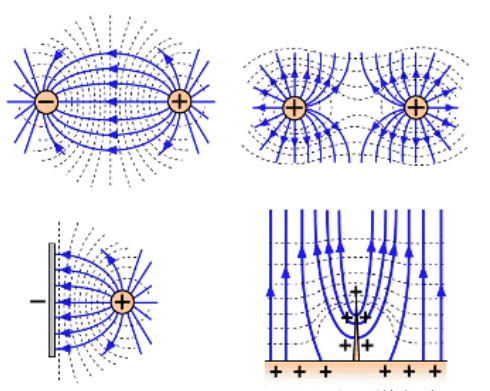
\includegraphics[scale=0.75]{1.png}

\end{document}